% \renewcommand{\imagewidth}{2.3cm}
\renewcommand{\imageheight}{4.5263671874999996cm}
\renewcommand{\smallimagewidth}{0.8cm}

\newcommand{\imageoneindex}[2]{
  \includegraphics[height=\imageheight, trim={0.7cm 1.8cm 0.7cm 0}, clip]{assets/\blendfieldsdirname/qualitative/extrapolation/#1_6795937_extrapolation_#2.png}
}
\newcommand{\imagetwoindex}[2]{
  \includegraphics[height=\imageheight, trim={1.4cm 1.8cm 0 0}, clip]{assets/\blendfieldsdirname/qualitative/extrapolation/#1_7889059_extrapolation_#2.png}
}
\renewcommand{\versionone}{
  \tikzsetnextfilename{blendfields_qualitative_comparison_extrapolation}
  \begin{tikzpicture}[
      >=stealth',
      overlay/.style={
          anchor=south west,
          draw=black,
          rectangle,
          line width=0.8pt,
          outer sep=0,
          inner sep=0,
        },
    ]
    \matrix[
      matrix of nodes,
      column sep=0pt,
      row sep=0pt,
      ampersand replacement=\&,
      inner sep=0,
      outer sep=0
    ] (nerf) {
      \imageoneindex{nerf}{0000} \\
      % \imageoneindex{nerf}{0002} \\
      \imageoneindex{nerf}{0004} \\

      \imagetwoindex{nerf}{0000} \\
      % \imagetwoindex{nerf}{0002} \\
      \imagetwoindex{nerf}{0004} \\
    };

    \matrix[
      matrix of nodes,
      column sep=0pt,
      row sep=0pt,
      ampersand replacement=\&,
      inner sep=0,
      outer sep=0,
      right=1pt of nerf
    ] (dnerf) {
      \imageoneindex{dnerf}{0000} \\
      % \imageoneindex{dnerf}{0002} \\
      \imageoneindex{dnerf}{0004} \\

      \imagetwoindex{dnerf}{0000} \\
      % \imagetwoindex{dnerf}{0002} \\
      \imagetwoindex{dnerf}{0004} \\
    };

    \matrix[
      matrix of nodes,
      column sep=0pt,
      row sep=0pt,
      ampersand replacement=\&,
      inner sep=0,
      outer sep=0,
      right=1pt of dnerf
    ] (nerfies) {
      \imageoneindex{nerfies}{0000} \\
      % \imageoneindex{nerfies}{0002} \\
      \imageoneindex{nerfies}{0004} \\

      \imagetwoindex{nerfies}{0000} \\
      % \imagetwoindex{nerfies}{0002} \\
      \imagetwoindex{nerfies}{0004} \\
    };

    \matrix[
      matrix of nodes,
      column sep=0pt,
      row sep=0pt,
      ampersand replacement=\&,
      inner sep=0,
      outer sep=0,
      right=1pt of nerfies
    ] (hypernerfstatic) {
      \imageoneindex{hypernerf_static}{0000} \\
      % \imageoneindex{hypernerf_static}{0002} \\
      \imageoneindex{hypernerf_static}{0004} \\

      \imagetwoindex{hypernerf_static}{0000} \\
      % \imagetwoindex{hypernerf_static}{0002} \\
      \imagetwoindex{hypernerf_static}{0004} \\
    };

    \matrix[
      matrix of nodes,
      column sep=0pt,
      row sep=0pt,
      ampersand replacement=\&,
      inner sep=0,
      outer sep=0,
      right=1pt of hypernerfstatic
    ] (hypernerfdynamic) {
      \imageoneindex{hypernerf_dynamic}{0000} \\
      % \imageoneindex{hypernerf_dynamic}{0002} \\
      \imageoneindex{hypernerf_dynamic}{0004} \\

      \imagetwoindex{hypernerf_dynamic}{0000} \\
      % \imagetwoindex{hypernerf_dynamic}{0002} \\
      \imagetwoindex{hypernerf_dynamic}{0004} \\
    };

    \matrix[
      matrix of nodes,
      column sep=0pt,
      row sep=0pt,
      ampersand replacement=\&,
      inner sep=0,
      outer sep=0,
      right=1pt of hypernerfdynamic
    ] (voltemorphstatic) {
      \imageoneindex{voltemorph_static}{0000} \\
      % \imageoneindex{voltemorph_static}{0002} \\
      \imageoneindex{voltemorph_static}{0004} \\

      \imagetwoindex{voltemorph_static}{0000} \\
      % \imagetwoindex{voltemorph_static}{0002} \\
      \imagetwoindex{voltemorph_static}{0004} \\
    };

    \matrix[
      matrix of nodes,
      column sep=0pt,
      row sep=0pt,
      ampersand replacement=\&,
      inner sep=0,
      outer sep=0,
      right=1pt of voltemorphstatic
    ] (voltemorph) {
      \imageoneindex{voltemorph}{0000} \\
      % \imageoneindex{voltemorph}{0002} \\
      \imageoneindex{voltemorph}{0004} \\

      \imagetwoindex{voltemorph}{0000} \\
      % \imagetwoindex{voltemorph}{0002} \\
      \imagetwoindex{voltemorph}{0004} \\
    };

    \matrix[
      matrix of nodes,
      column sep=0pt,
      row sep=0pt,
      ampersand replacement=\&,
      inner sep=0,
      outer sep=0,
      right=1pt of voltemorph
    ] (ours) {
      \imageoneindex{blendvolumes_aux}{0000} \\
      % \imageoneindex{blendvolumes_aux}{0002} \\
      \imageoneindex{blendvolumes_aux}{0004} \\

      \imagetwoindex{blendvolumes_aux}{0000} \\
      % \imagetwoindex{blendvolumes_aux}{0002} \\
      \imagetwoindex{blendvolumes_aux}{0004} \\
    };
    \node[above=0.2em of nerf-1-1.north, align=center, anchor=south]{NeRF};
    \node[above=0.2em of dnerf-1-1.north, align=center, anchor=south]{Conditioned NeRF};
    \node[above=0.2em of nerfies-1-1.north, align=center, anchor=south]{NeRFies};
    \node[above=0.0em of hypernerfstatic-1-1.north, align=center, anchor=south]{HyperNeRF-AP};
    \node[above=0.0em of hypernerfdynamic-1-1.north, align=center, anchor=south]{HyperNeRF-DS};
    \node[above=0.0em of voltemorphstatic-1-1.north, align=center, anchor=south]{VolTeMorph$^\dagger$};
    \node[above=0.0em of voltemorph-1-1.north, align=center, anchor=south]{VolTeMorph};
    \node[above=0.2em of ours-1-1.north, align=center, anchor=south]{\textbf{Ours}};

    \node[left=0em of nerf-1-1.west, align=center, anchor=east]{\rotatebox{90}{Neutral}};
    \node[left=0em of nerf-3-1.west, align=center, anchor=east]{\rotatebox{90}{Neutral}};

    \node[left=0em of nerf-2-1.west, align=center, anchor=east]{\rotatebox{90}{Frowned and Smile}};
    \node[left=0em of nerf-4-1.west, align=center, anchor=east]{\rotatebox{90}{Eyes Squint, Lips Moved Left}};
  \end{tikzpicture}
}

\begin{figure*}[htb]
  \centering
  \resizebox{\linewidth}{!}{
    \versionone
  }
  % \includegraphics[height=0.75\textheight, width=\linewidth]{example-image-a}
  \caption{\textbf{Novel expression synthesis} --
    We compare qualitatively \blendfields with selected baselines (horizontal) across two selected subjects (vertical).
    As clearly seen, our approach renders the most realistic frames given any
    of the expressions.
    VolTeMorph, while being capable of rendering already realistic, controlled
    images, it cannot capture expression-dependent details.
    In contrast, \blendfields captures these details and generalizes outside
    of the distribution.
    Please refer to the \supplementary{} for animated sequences and results
    for other methods.
  }
  \label{fig:blendfields-qualitative-comparison}
\end{figure*}
% !TEX program = xelatex

%%%%%%%%%%%%%%%%%%%%%%%%%%%%%%%%%%%%%%%%%%%%%%%%%%%%%%%%%%%%%%%%%%%%%%%%%%%
% Wybierz rodzaj pracy dyplomowej oraz wydział
% Pick thesis type and faculty
%%%%%%%%%%%%%%%%%%%%%%%%%%%%%%%%%%%%%%%%%%%%%%%%%%%%%%%%%%%%%%%%%%%%%%%%%%%
\documentclass{diploma} 
\instytut{Faculty of Electronics and Information Technology}
\dyscyplina{Information and Communication Technology}
\title{Renderowanie Ludzi z Kilku Próbek z Użyciem Częściowej Informacji}
\engtitle{Few-Shot Human Neural Rendering with Partial Information}
\album{KD-277}
\author{mgr inż. Kacper Kania}
\promotor{prof. dr hab. inż. Tomasz Trzciński}
\promotorpomocniczy{dr hab. inż. Marek Kowalski}
\date{2025}
\longdate{2025-01-01}


%\grantlicense{TRUE} % [TRUE|FALSE]

%%%%%%%%%%%%%%%%%%%%%%%%%%%%%%%%%%%%%%%%%%%%%%%%%%%%%%%%%%%%%%%%%%%%%%%%%%%
% Streszczenie pracy i abstract.
% In case of thesis in English swap the order - English version goes first.

%%%%%%%%%%%%%%%%%%%%%%%%%%%%%%%%%%%%%%%%%%%%%%%%%%%%%%%%%%%%%%%%%%%%%%%%%%%
\streszczeniepracy{
To jest streszczenie. To jest trochę za krótkie, jako że powinno zająć całą stronę.
\lipsum[1-4]
} % koniec streszczenia

\slowakluczowe{A, B, C}

\thesisabstract{
This is abstract. This one is a little too short as it should occupy the whole page.

\lipsum[1-4]
} % end of abstract





\thesiskeywords{X, Y, Z}

%%%%%%%%%%%%%%%%%%%%%%%%%%%%%%%%%%%%%%%%%%%%%%%%%%%%%%%%%%%%%%%%%%%%%%%%%%%
% Tu zaczyna się dokument
% Here is the beginning of the document
%%%%%%%%%%%%%%%%%%%%%%%%%%%%%%%%%%%%%%%%%%%%%%%%%%%%%%%%%%%%%%%%%%%%%%%%%%%
\begin{document}
    % Headers
    \frontpages


    % Właściwa treść jest w pliku tekst/main.tex
    % Real contents is in tekst/main.tex
    % % !TEX program = xelatex

%%%%%%%%%%%%%%%%%%%%%%%%%%%%%%%%%%%%%%%%%%%%%%%%%%%%%%%%%%%%%%%%%%%%%%%%%%%
% Wybierz rodzaj pracy dyplomowej oraz wydział
% Pick thesis type and faculty
%%%%%%%%%%%%%%%%%%%%%%%%%%%%%%%%%%%%%%%%%%%%%%%%%%%%%%%%%%%%%%%%%%%%%%%%%%%
\documentclass{diploma} 
\instytut{Faculty of Electronics and Information Technology}
\dyscyplina{Information and Communication Technology}
\title{Renderowanie Ludzi z Kilku Próbek z Użyciem Częściowej Informacji}
\engtitle{Few-Shot Human Neural Rendering with Partial Information}
\album{KD-277}
\author{mgr inż. Kacper Kania}
\promotor{prof. dr hab. inż. Tomasz Trzciński}
\promotorpomocniczy{dr hab. inż. Marek Kowalski}
\date{2025}
\longdate{2025-01-01}


%\grantlicense{TRUE} % [TRUE|FALSE]

%%%%%%%%%%%%%%%%%%%%%%%%%%%%%%%%%%%%%%%%%%%%%%%%%%%%%%%%%%%%%%%%%%%%%%%%%%%
% Streszczenie pracy i abstract.
% In case of thesis in English swap the order - English version goes first.

%%%%%%%%%%%%%%%%%%%%%%%%%%%%%%%%%%%%%%%%%%%%%%%%%%%%%%%%%%%%%%%%%%%%%%%%%%%
\streszczeniepracy{
To jest streszczenie. To jest trochę za krótkie, jako że powinno zająć całą stronę.
\lipsum[1-4]
} % koniec streszczenia

\slowakluczowe{A, B, C}

\thesisabstract{
This is abstract. This one is a little too short as it should occupy the whole page.

\lipsum[1-4]
} % end of abstract





\thesiskeywords{X, Y, Z}

%%%%%%%%%%%%%%%%%%%%%%%%%%%%%%%%%%%%%%%%%%%%%%%%%%%%%%%%%%%%%%%%%%%%%%%%%%%
% Tu zaczyna się dokument
% Here is the beginning of the document
%%%%%%%%%%%%%%%%%%%%%%%%%%%%%%%%%%%%%%%%%%%%%%%%%%%%%%%%%%%%%%%%%%%%%%%%%%%
\begin{document}
    % Headers
    \frontpages


    % Właściwa treść jest w pliku tekst/main.tex
    % Real contents is in tekst/main.tex
    % % !TEX program = xelatex

%%%%%%%%%%%%%%%%%%%%%%%%%%%%%%%%%%%%%%%%%%%%%%%%%%%%%%%%%%%%%%%%%%%%%%%%%%%
% Wybierz rodzaj pracy dyplomowej oraz wydział
% Pick thesis type and faculty
%%%%%%%%%%%%%%%%%%%%%%%%%%%%%%%%%%%%%%%%%%%%%%%%%%%%%%%%%%%%%%%%%%%%%%%%%%%
\documentclass{diploma} 
\instytut{Faculty of Electronics and Information Technology}
\dyscyplina{Information and Communication Technology}
\title{Renderowanie Ludzi z Kilku Próbek z Użyciem Częściowej Informacji}
\engtitle{Few-Shot Human Neural Rendering with Partial Information}
\album{KD-277}
\author{mgr inż. Kacper Kania}
\promotor{prof. dr hab. inż. Tomasz Trzciński}
\promotorpomocniczy{dr hab. inż. Marek Kowalski}
\date{2025}
\longdate{2025-01-01}


%\grantlicense{TRUE} % [TRUE|FALSE]

%%%%%%%%%%%%%%%%%%%%%%%%%%%%%%%%%%%%%%%%%%%%%%%%%%%%%%%%%%%%%%%%%%%%%%%%%%%
% Streszczenie pracy i abstract.
% In case of thesis in English swap the order - English version goes first.

%%%%%%%%%%%%%%%%%%%%%%%%%%%%%%%%%%%%%%%%%%%%%%%%%%%%%%%%%%%%%%%%%%%%%%%%%%%
\streszczeniepracy{
To jest streszczenie. To jest trochę za krótkie, jako że powinno zająć całą stronę.
\lipsum[1-4]
} % koniec streszczenia

\slowakluczowe{A, B, C}

\thesisabstract{
This is abstract. This one is a little too short as it should occupy the whole page.

\lipsum[1-4]
} % end of abstract





\thesiskeywords{X, Y, Z}

%%%%%%%%%%%%%%%%%%%%%%%%%%%%%%%%%%%%%%%%%%%%%%%%%%%%%%%%%%%%%%%%%%%%%%%%%%%
% Tu zaczyna się dokument
% Here is the beginning of the document
%%%%%%%%%%%%%%%%%%%%%%%%%%%%%%%%%%%%%%%%%%%%%%%%%%%%%%%%%%%%%%%%%%%%%%%%%%%
\begin{document}
    % Headers
    \frontpages


    % Właściwa treść jest w pliku tekst/main.tex
    % Real contents is in tekst/main.tex
    % \input{tekst/main}

    % % Bibliografia - musi być
    % % Bibliography - must exist
    % \bibliografia

    % % Strony końcowe - można zakomentować, jeśli zbędne
    % % Additional pages - comment out if not needed
    
    % % Wykaz symboli i skrótów - patrz opis w tekście przykładowym
    \acronymslist
    % % % Spis rysunków
    % \listoffigures
    % % % Spis tabel
    % \listoftables
    % % % Załączniki (plik appendices.tex)
    % \easyappendices
\end{document}
%%%%%%%%%%%%%%%%%%%%%%%%%%%%%%%%%%%%%%%%%%%%%%%%%%%%%%%%%%%%%%%%%%%%%%%%%%%



    % % Bibliografia - musi być
    % % Bibliography - must exist
    % \bibliografia

    % % Strony końcowe - można zakomentować, jeśli zbędne
    % % Additional pages - comment out if not needed
    
    % % Wykaz symboli i skrótów - patrz opis w tekście przykładowym
    \acronymslist
    % % % Spis rysunków
    % \listoffigures
    % % % Spis tabel
    % \listoftables
    % % % Załączniki (plik appendices.tex)
    % \easyappendices
\end{document}
%%%%%%%%%%%%%%%%%%%%%%%%%%%%%%%%%%%%%%%%%%%%%%%%%%%%%%%%%%%%%%%%%%%%%%%%%%%



    % % Bibliografia - musi być
    % % Bibliography - must exist
    % \bibliografia

    % % Strony końcowe - można zakomentować, jeśli zbędne
    % % Additional pages - comment out if not needed
    
    % % Wykaz symboli i skrótów - patrz opis w tekście przykładowym
    \acronymslist
    % % % Spis rysunków
    % \listoffigures
    % % % Spis tabel
    % \listoftables
    % % % Załączniki (plik appendices.tex)
    % \easyappendices
\end{document}
%%%%%%%%%%%%%%%%%%%%%%%%%%%%%%%%%%%%%%%%%%%%%%%%%%%%%%%%%%%%%%%%%%%%%%%%%%%



\begin{table*}[!t]
  \centering
  \resizebox{\linewidth}{!}{
    \begin{tabular}{lccccccccc}
      \toprule
      \multirow{3}[3]{*}{Parameter}    & \multicolumn{6}{c}{Real Data}          & \multicolumn{3}{c}{Synthetic Data}                                                                                                                                                                                                                                                                            \\
      \cmidrule(lr){2-7}\cmidrule(lr){8-10}
                                       & \multicolumn{3}{c}{Casual Expressions} & \multicolumn{3}{c}{Novel Pose Synthesis} & \multicolumn{3}{c}{Novel Pose Synthesis}                                                                                                                                                                                                                           \\
      \cmidrule(lr){2-4}\cmidrule(lr){5-7}\cmidrule(lr){8-10}
                                       & PSNR $\uparrow$                        & SSIM $\uparrow$                          & LPIPS $\downarrow$                       & PSNR $\uparrow$                    & SSIM $\uparrow$                   & LPIPS $\downarrow$                & PSNR $\uparrow$                    & SSIM $\uparrow$                   & LPIPS $\downarrow$                \\
      \midrule
      $|\neighbourhood(\vertex)| = 1$  & 27.5620                                & 0.9043                                   & 0.0893                                   & 29.7269                            & 0.9306                            & 0.0815                            & 32.2371                            & \cellcolor{secondbestcolor}0.9882 & 0.0234                            \\
      $|\neighbourhood(\vertex)| = 5$  & 27.5880                                & \cellcolor{secondbestcolor}0.9054        & 0.0864                                   & \cellcolor{firstbestcolor}29.7548  & \cellcolor{secondbestcolor}0.9312 & 0.0789                            & 32.2900                            & \cellcolor{secondbestcolor}0.9882 & 0.0231                            \\
      $|\neighbourhood(\vertex)| = 10$ & \cellcolor{secondbestcolor}27.5933     & \cellcolor{secondbestcolor}0.9054        & \cellcolor{secondbestcolor}0.0859        & \cellcolor{secondbestcolor}29.7456 & \cellcolor{secondbestcolor}0.9312 & \cellcolor{secondbestcolor}0.0785 & \cellcolor{secondbestcolor}32.3324 & \cellcolor{secondbestcolor}0.9882 & \cellcolor{secondbestcolor}0.0230 \\
      $|\neighbourhood(\vertex)| = 20$ & \cellcolor{firstbestcolor}27.5977      & \cellcolor{firstbestcolor}0.9056         & \cellcolor{firstbestcolor}0.0854         & 29.7372                            & 0.9311                            & \cellcolor{firstbestcolor}0.0782  & \cellcolor{firstbestcolor}32.7949  & \cellcolor{firstbestcolor}0.9887  & \cellcolor{firstbestcolor}0.0221  \\
      \midrule
      Without smoothing                & \cellcolor{secondbestcolor}27.2535     & \cellcolor{secondbestcolor}0.8959        & \cellcolor{secondbestcolor}0.0939        & \cellcolor{secondbestcolor}29.3726 & \cellcolor{secondbestcolor}0.9233 & \cellcolor{secondbestcolor}0.0846 & \cellcolor{secondbestcolor}32.2452 & \cellcolor{secondbestcolor}0.9876 & \cellcolor{secondbestcolor}0.0238 \\
      With smoothing                   & \cellcolor{firstbestcolor}27.5977      & \cellcolor{firstbestcolor}0.9056         & \cellcolor{firstbestcolor}0.0854         & \cellcolor{firstbestcolor}29.7372  & \cellcolor{firstbestcolor}0.9311  & \cellcolor{firstbestcolor}0.0782  & \cellcolor{firstbestcolor}32.7949  & \cellcolor{firstbestcolor}0.9887  & \cellcolor{firstbestcolor}0.0221  \\
      \bottomrule
    \end{tabular}
  }
  \caption{\textbf{Ablation study} -- {
  First, we check the effect of the neighborhood size $|\neighbourhood(\vertex)|$ on the results.
  Below that, we compare the effect of smoothing.
  % We highlight ablations results as its the only benchmark where the
  % deformable model is fit reliably. 
  The best results are colored in \mycoloredbox{firstbestcolor} and the second
  best in \mycoloredbox{secondbestcolor}.
  For the real dataset, changing the neighborhood size gives inconsistent
  results, while smoothing improves the rendering quality.
  In the synthetic scenario, setting $|\neighbourhood(\vertex)|{=}20$ and the
  Laplacian smoothing consistently gives the best results.
  The discrepancy between real and synthetic datasets is caused by inaccurate
  face tracking for the former.
  We describe this issue in detail in~\cref{subsec:blendfields-failures}.
  }
  }
  \label{tab:blendfields-ablation-study}
\end{table*}

\renewcommand{\imagewidth}{2.3cm}
\renewcommand{\imageheight}{4.0cm}
\renewcommand{\smallimagewidth}{0.8cm}
\newcommand{\borderwidth}{2.0pt}
\newcommand{\spacingbetweencols}{2.0pt}

\newcommand{\imageindex}[2]{
  \includegraphics[height=\imageheight, trim={4.6cm 1.5cm 4.6cm 1.5cm}, clip]{assets/\blendfieldsdirname/synthetics/#1_synthetic_#2}
}
\renewcommand{\versionone}{
  \begin{tikzpicture}[
      >=stealth',
      overlay/.style={
          anchor=south west,
          draw=black,
          rectangle,
          line width=0.8pt,
          outer sep=0,
          inner sep=0,
        },
    ]
    \matrix[
      matrix of nodes,
      column sep=0pt,
      row sep=0pt,
      ampersand replacement=\&,
      inner sep=0,
      outer sep=0,
      % draw=black, rectangle, line width=\borderwidth
    ] (main) {
      \imageindex{gt}{0000} \\
      \imageindex{gt}{0002} \\
    };
    \matrix[
      matrix of nodes,
      column sep=0pt,
      row sep=0pt,
      ampersand replacement=\&,
      inner sep=0,
      outer sep=0,
      % draw=red, rectangle, line width=\borderwidth,
      right=\spacingbetweencols of main
    ] (voltemorph) {
      \imageindex{voltemorph_static}{0000} \&
      \imageindex{voltemorph}{0000} \\
      \imageindex{voltemorph_static}{0002} \&
      \imageindex{voltemorph}{0002} \\
    };
    \matrix[
      matrix of nodes,
      column sep=0pt,
      row sep=0pt,
      ampersand replacement=\&,
      inner sep=0,
      outer sep=0,
      % draw=OliveGreen, rectangle, line width=\borderwidth,
      right=\spacingbetweencols of voltemorph
    ] (blendvolumes) {
      \imageindex{blendvolumes_aux}{0000} \\
      \imageindex{blendvolumes_aux}{0002} \\
    };

    \node[above=0.2em of main-1-1.north, align=center, anchor=south]{Ground Truth};
    \node[above=0.0em of voltemorph-1-1.north, align=center, anchor=south]{VolTeMorph$_1$};
    \node[above=0.0em of voltemorph-1-2.north, align=center, anchor=south]{VolTeMorph$_\text{avg}$};
    \node[above=0.1em of blendvolumes-1-1.north, align=center, anchor=south]{\textbf{Ours}};

    \node[left=0.1em of main-1-1.west, align=center, anchor=east]{\rotatebox{90}{Canonical}};
    \node[left=0.1em of main-2-1.west, align=center, anchor=east]{\rotatebox{90}{Twisted}};
  \end{tikzpicture}
}
\begin{figure}[t]
  \centering
  \resizebox{\linewidth}{!}{\versionone}
  \caption{\textbf{Qualitative results on synthetic dataset} --  For a simple dataset, baselines cannot model high-frequency, pose-dependent details.
    VolTeMorph$_1$ renders wrinkles for the straight pose as well, as it is
    trained for the twisted cylinder only, while VolTeMorph$_\text{avg}$
    averages out the texture.
  }
  \label{fig:blendfields-synthetic-qualitative}
\end{figure}

\section{Experiments}
  \label{sec:blendfields-experiments}

  We evaluate all methods on data of four subjects from the publicly available
  Multiface dataset~\cite{wuu2022multiface}.
  We track the face for eight manually-selected ''extreme'' expressions.
  We then select $\nExpr{=}5$ expressions the combinations of which show as
  many wrinkles as possible.
  Each subject was captured with $\approx\!
    \!38$ cameras which gives~$\approx\!\!190$ training images per subject
  \footnote{To train \blendfields for a single subject we use $\approx0.006\%$ of the dataset used by AVA~\cite{cao2022authentic}.}.
  We use Peak Signal To Noise Ratio (PSNR)~\cite{avcibas2002statistical},
  Structural Similarity Index (SSIM)~\cite{wang2003multiscale} and Learned
  Perceptual Image Patch Similarity (LPIPS)~\cite{zhang2018perceptual} to
  measure the performance of the models.
  Each of the rendered images has a resolution of $334{\times}512$ pixels.

  As baselines, we use the following approaches: the original, static
  NeRF~\cite{mildenhall2020nerf}, NeRF conditioned on an expression code
  concatenated with input points~$\pos$, NeRFies~\cite{park2021nerfies},
  HyperNeRF\footnote{We use two architectures proposed by
  Park~\etal~\cite{park2021hypernerf}.
  }~\cite{park2021hypernerf}, and VolTeMorph~\cite{garbin2024voltemorph}.
  We replace the learnable code in NeRFies and HyperNeRF with the expression
  code $\expression$ from the parametric model.
  Since VolTeMorph can be trained on multiple frames, which should lead to
  averaging of the output colors, we split it into two regimes: one trained on
  the most extreme expression\footnote{We manually select one frame that has
  the most visible wrinkles.
  } (VolTeMorph$_1$) and the another trained on all available expressions (VolTeMorph$_\text{avg}$)\footnote{We do not compare to NeRFace~\cite{gafni2021dynamic} and NHA~\cite{neural_head_avatars} as VolTeMorph~\cite{garbin2024voltemorph} performs better quantitatively than these methods.}.
  We use both of these baselines as VolTeMorph was originally designed for a
  single-frame scenario.
  By using two versions, we show that it is not trivial to extend it to
  multiple expressions.

  \subsection{Realistic Human Captures}
    \label{subsec:blendfields-realistic-human-captures}
    \noindent\textbf{Novel expression synthesis.}
    We extract eight multi-view frames from the Multiface
    dataset~\cite{wuu2022multiface}, each of a different expression.
    Five of these expressions serve as training data, and the rest are used
    for evaluation.
    After training, we can extrapolate from the training expressions by
    modifying the expression vector~$\expression$.
    We use the remaining three expressions: moving mouth left and right, and
    puffing cheeks, to evaluate the capability of the models to reconstruct
    other expressions.
    % the sentence below was originally before the one above
    In~\cref{fig:blendfields-qualitative-comparison} we show that \blendfields
    is the only method capable of rendering convincing wrinkles dynamically,
    depending on the input expression.
    % In that scenario, 
    \blendfields performs favorably compared to the baselines~(see \cref{tab:blendfields-quantitative-results}).

    \noindent\textbf{Casual expressions.}
    The Multiface dataset contains sequences where the subject follows a
    script of expressions to show during the capture.
    Each of these captures contains between 1000 and 2000 frames.
    This experiment tests whether a model can interpolate between the training
    expressions smoothly and generalize beyond the training data.
    Quantitative results are shown in
    \cref{tab:blendfields-quantitative-results}.
    Our approach performs best all the settings.
    See animations in the \supplementary{} for a comparison of rendered frames
    across all methods.

  \subsection{Modeling Objects Beyond Faces}
    We show that our method can be applied beyond face modeling.
    We prepare two datasets containing 96 views per frame of bending and
    twisting cylinders made of a rubber-like material (24 and 72 temporal
    frames, respectively).
    When bent or twisted, the cylinders reveal pose-dependent details.
    The expression vector $\expression$ now encodes time: 0 if the cylinder is
    in the canonical pose, 1 if it is posed, and any values between $[0, 1]$
    for the transitioning stage.
    We select expressions $\{0, 0.5, 1.0\}$ as a training set (for
    VolTeMorph$_1$ we use $1.0$ only).
    For evaluation, we take every fourth frame from the full sequence using
    cameras from the bottom and both sides of the object.
    We take the mesh directly from Houdini~\cite{xu2014houdini}, which we use
    for wrinkle simulation, and render the images in
    Blender~\cite{blender2022}.
    We show quantitative results
    in~\cref{tab:blendfields-quantitative-results} for the bending cylinder,
    and a comparison of the inferred images
    in~\cref{fig:blendfields-synthetic-qualitative} for the twisted
    one\footnote{Our motivation is that it is easier to show pose-dependent
    deformations on twisting as it affects the object globally, while the
    bending cannot be modeled by all the baselines due to the non-stationary
    effects.
    }. \blendfields accurately captures the transition from the rest configuration to the deformed state of the cylinder, rendering high-frequency details where required.
    All other approaches struggle with interpolation between states.
    VolTeMorph$_1$ (trained on a single extreme pose) renders wrinkles even
    when the cylinder is not twisted.

  \subsection{Ablations}
    We check how the neighborhood size~$|\neighbourhood(\vertex)|$ and the
    application of the smoothing influence the performance of our method.
    We show the results in~\cref{tab:ablation-study}.
    \blendfields works best in most cases when considering a relatively wide neighborhood for the tetrahedral features\footnote{Larger neighborhood sizes caused out-of-memory errors on our NVIDIA 2080Ti GPU.}.
    Laplacian smoothing consistently improves the quality across all the
    datasets~(see~\cref{fig:blendfields-laplacian-smoothing}).
    We additionally present in the \supplementary{} how the number of
    expressions used for training affects the results.

  \subsection{Failure Cases}
    \label{subsec:blendfields-failures}
    \newcommand{\leftimageheight}{4.5cm}
\newcommand{\rightimageheight}{4.5cm}

\renewcommand{\versionone}{
  \begin{tikzpicture}[
      >=stealth',
      overlay/.style={
          anchor=south west,
          draw=black,
          rectangle,
          line width=0.8pt,
          outer sep=0,
          inner sep=0,
        },
    ]
    \matrix[
      matrix of nodes,
      column sep=2pt,
      row sep=0pt,
      ampersand replacement=\&,
      inner sep=0,
      outer sep=0,
    ] (main) {
      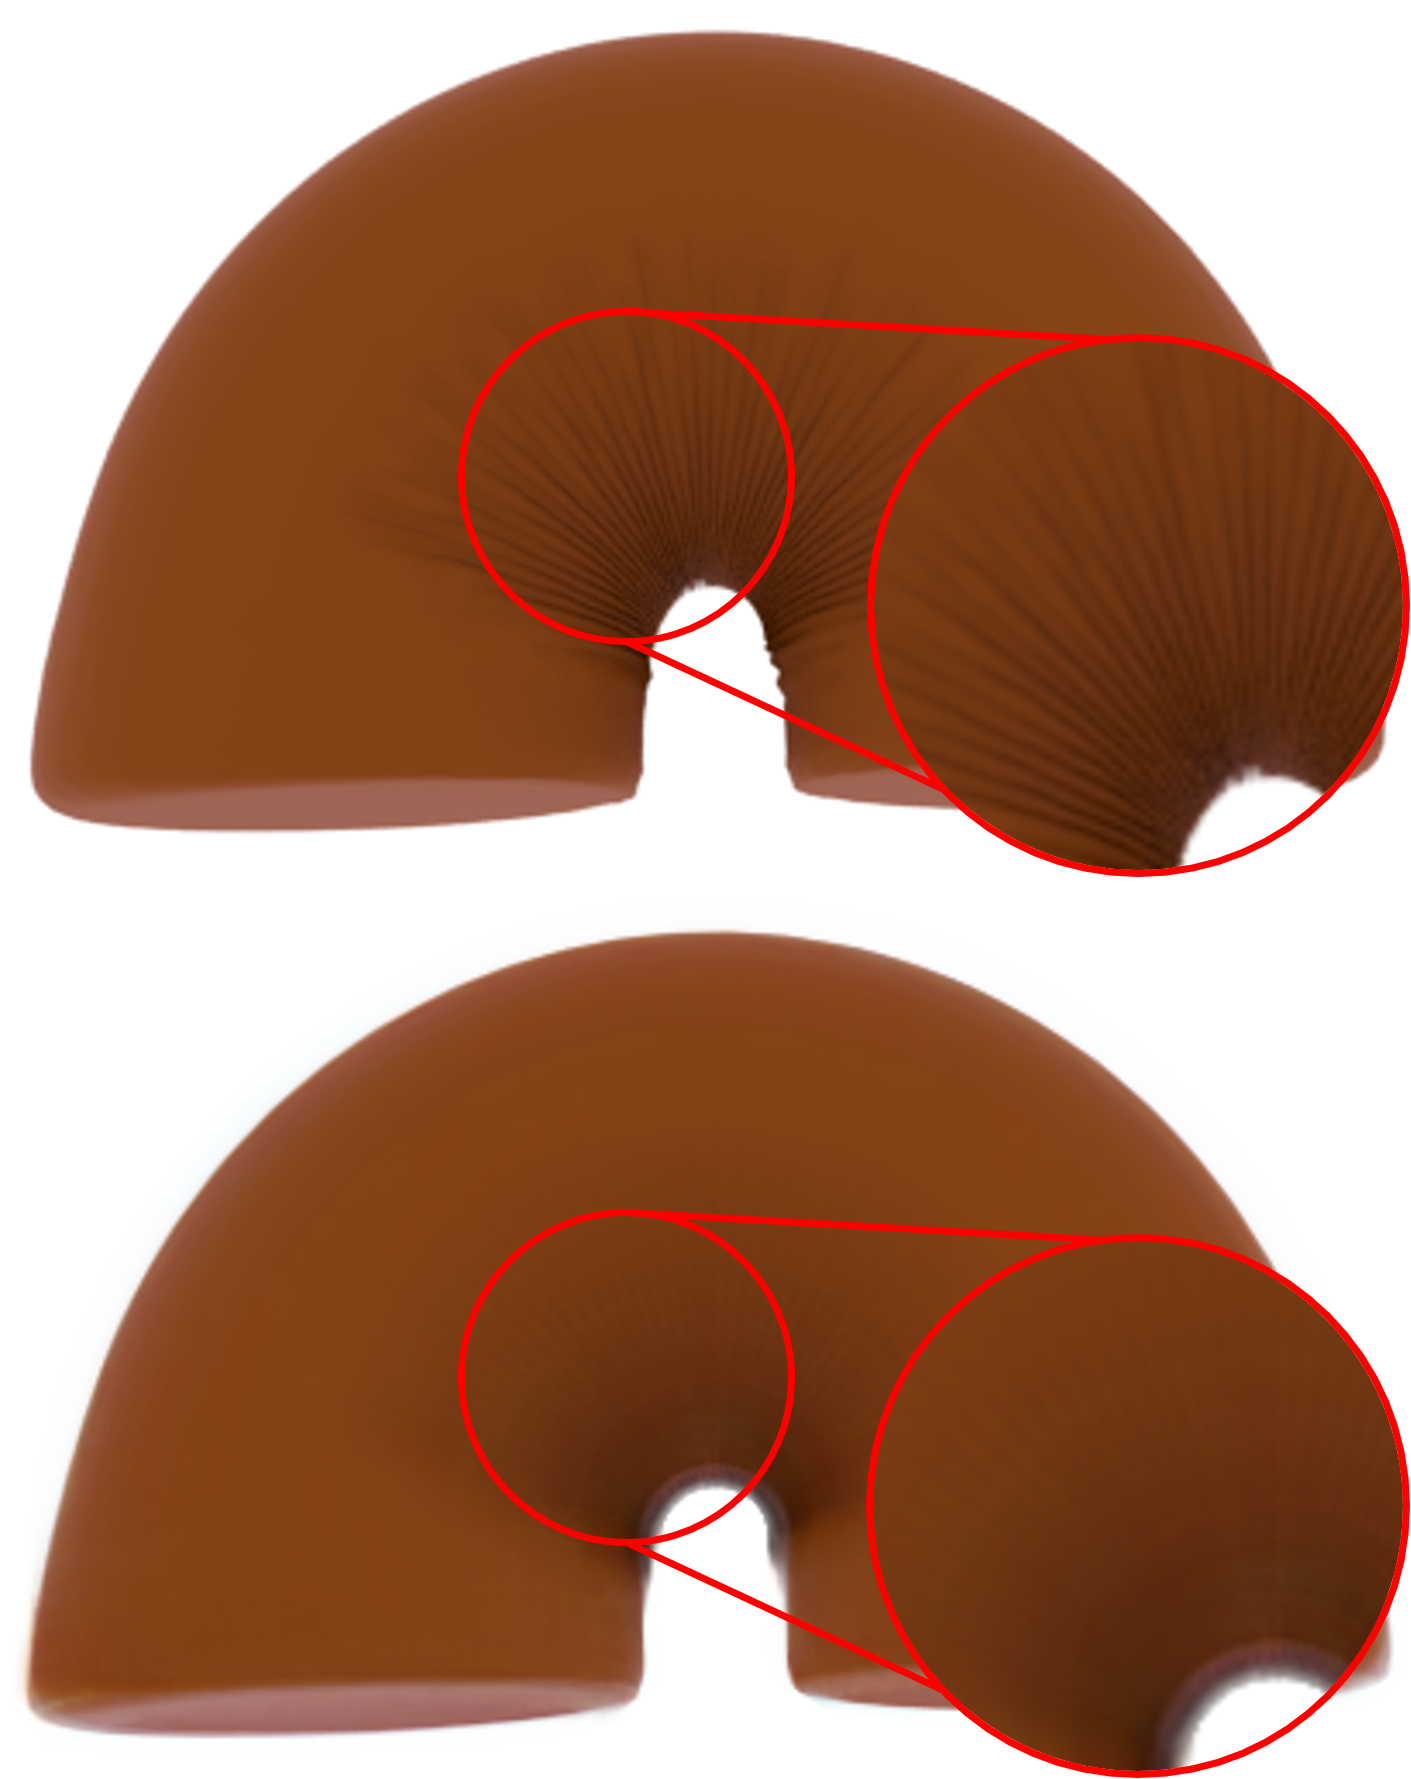
\includegraphics[height=\leftimageheight]{assets/\blendfieldsdirname/failures/convergence.png} \&
      \includegraphics[height=\rightimageheight]{assets/\blendfieldsdirname/failures/tracking.png} \\
    };
    \node[above=0.0em of main-1-1.north, align=center, anchor=south]{Low contrast};
    \node[above=0.0em of main-1-2.north, align=center, anchor=south]{Inaccurate off-the-shelf tracker};
  \end{tikzpicture}
}
\begin{figure}[t]
  \centering
  \resizebox{0.7\linewidth}{!}{\versionone}
  \caption{\textbf{Failure cases} -- {
      We show failure cases for our proposed approach.
      \textit{Left:}
      In the presence of wrinkles in low-contrast images, \blendfields takes
      longer to converge to make wrinkles visible.
      We show the ground truth on the top, and rendering after training
      $7{\times}10^5$ steps on the bottom.
      In contrast, we rendered images
      in~\cref{fig:blendfields-synthetic-qualitative} after $2{\times}10^5$
      steps.
      \textit{Right:} \blendfields inherits issues from VolTeMorph~\cite{garbin2024voltemorph}, which relies on the initial fit of the face mesh.
      If the fit is inaccurate, artifacts appear in the final render.
    }}
  \label{fig:blendfields-failure-cases}
\end{figure}
    While \blendfields offers significant advantages for rendering realistic
    and dynamic high-frequency details, it falls short in some scenarios
    (see~\cref{fig:blendfields-failure-cases}).
    One of the issues arises when the contrast between wrinkles and the
    subject's skin color is low.
    In those instances, we observe a much longer time to convergence.
    Moreover, as we build \blendfields on VolTeMorph, we also inherit some of
    its problems.
    Namely, the method heavily relies on the initial fit of the parametric
    model---any inaccuracy leads to ghosting artifacts or details on the face
    that jump between frames.
